\section{Mechanics}

\subsection{Overview of common physical quantities}

\begin{figure}[H]
\centering
    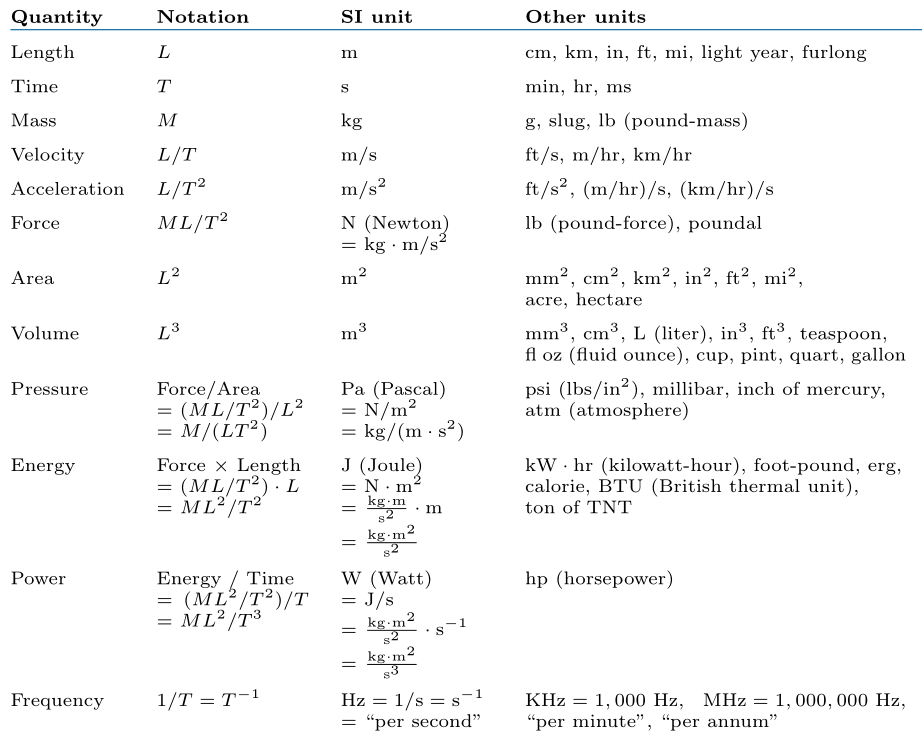
\includegraphics[width=\textwidth]{11_physical_quantities}
\caption{Selected physicial quantities}
\label{fig:physical-quantities}
\end{figure}

Velocity is a vector of displacement, while speed is a scalar of the rate at which an object is moving. The derivative measures the rate of change, since velocity measures the rate of change of position with respect to time, the velocity function is the derivative of the position function.

\subsection{Taylor series}

\begin{itemize}
	\item $\sin x = x - \frac{x^3}{3!} + \frac{x^5}{5!} - \frac{x^7}{7!} + \frac{x^9}{9!} + \dots$
	\item $\cos x = 1 - \frac{x^2}{2!} + \frac{x^4}{4!} - \frac{x^6}{6!} + \frac{x^8}{8!} + \dots$
	\item $e^x = 1 + x + \frac{x^2}{2!} + \frac{x^3}{3!} + \frac{x^4}{4!} + \dots$
\end{itemize}

Taking the derivatives and integrals from these series makes the derivatives definitions very obvious.

\subsection{Derivative definition}

$$\frac{dy}{dx}=\lim_{h \to 0} \frac{y(x+h)-y(x)}{h}$$

\subsection{Common derivatives}

\begin{itemize}
	\item $\frac{d}{dx}\sin x = \cos x$
	\item $\frac{d}{dx}\cos x = -\sin x$
	\item $\frac{d}{dx}e^x = e^x$
\end{itemize}